\documentclass{beamer}

\usetheme{Warsaw}

\usepackage{amsthm}
\usepackage{verbatim}
\usepackage{xcolor}
\usepackage{listings}
\usepackage{color}
\usepackage[utf8]{inputenc}
\usepackage[T1]{fontenc}
\usepackage{textcomp}
\usepackage{graphicx}
\usepackage[bulgarian]{babel}

\usepackage{hyperref}

\title{Въведение в Java, типове данни, масиви и оператори в Java, оператори if-else, switch, цикли, стандартен вход и изход, вход и изход - работа с файлове.}
\author{Валентин Гелински}
\institute{ТУ София}
\date{\today} 


\begin{document}


  \begin{frame} 
    \titlepage
  \end{frame}

  \section{За курса} 
  \subsection{Елементи на курса}

  \begin{frame} 
    \frametitle{Елементи на курса}
     \begin{tabular}{|c|c|c|c|}
       \hline
       Компонент&Периодичност&Брой&Точки\\
       \hline
       Присъствие&всяка седмица&8&2/упр\\
       \hline
       Домашни&равномерно&4&6/домашно\\
       \hline
       Контролно 1&веднъж&1&20\\
       \hline
       Контролно2&веднъж&1&40\\
       \hline
     \end{tabular}
  \end{frame}

  \subsection{Оценяване}

  \begin{frame}
    \frametitle{Оценяване}
    \begin{tabular}{|c|c|}
      \hline
      Точки&оценка\\
      \hline
      0-60&2\\
      \hline
      61-70&3\\
      \hline
      71-80&4\\
      \hline
      81-90&5\\
      \hline
      91-100&6\\
      \hline
    \end{tabular}
  \end{frame}

  \subsection{Друго}

  \begin{frame}
    \frametitle{Друго}
    \begin{itemize}
      \item{Wifi pass: fksu1211HALL}
      \item{\href{http://cphpvb.net/category/java/}{cphpvb.net}}
      \item{\href{https://www.facebook.com/groups/617381621641455/}{facebook}}
      \item{\href{https://github.com/vgelinski/tu_java_course}{github}}
    \end{itemize}
  \end{frame}

  \section{За мен}

  \begin{frame}
    \frametitle{За мен}
    \begin{itemize}
      \item{Валентин Гелински}
      \item{\href{mailto:gelinski.v@gmail.com}{gelinski.v@gmail.com}}
      \item{0888 318 047}
    \end{itemize}
  \end{frame}

  \section{Въведение в Java}
  \subsection{Началото}

  \begin{frame}
    \frametitle{Въведение в Java}
    Java е език за програмиране, създаден през 1991г. Първоначално под името Oak, а след 1995г преименуван в Java. Oak (от англ. - дъб) идва да покаже колко дървен е езика.
    \begin{itemize}
      \item{Обектно ориентиран}
      \item{Многоплатформен}
    \end{itemize}
  \end{frame}

  \subsection{Под капака}

  \begin{frame}
    \frametitle{Под капака}
    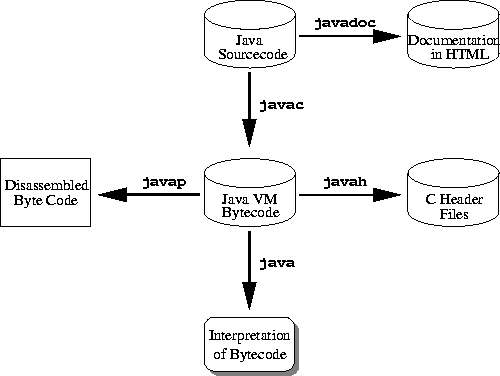
\includegraphics[width=250px]{img/img34}
  \end{frame}

  \subsection{Среди за разработка}

  \begin{frame}
    \frametitle{IDE в нужда се познава}
    \begin{itemize}
      \item{\href{http://drjava.org/}{Dr. Java}}
      \item{\href{https://netbeans.org}{NetBeans}}
      \item{\href{http://www.eclipse.org/home/index.php}{Eclipse}}
      \item{\href{http://www.jetbrains.com/idea/}{Idea}}
    \end{itemize}
  \end{frame}

  \subsection{Новото в Java}

  \begin{frame}
    \frametitle{Новото в Java}
    \begin{itemize}
      \item{Масиви (array)}
      \item{for-each}
      \item{go to, но не съвсем}
    \end{itemize}
  \end{frame}

  \section{Стандартен вход и изход}
  \subsection{Потоци}

  \begin{frame}
    \frametitle{Потоци}
    Потоците са връзката на програмата с външния свят.
  \end{frame}

  \subsection{Стандартни вход и изход}

  \begin{frame}
    \frametitle{Стандартни вход и изход}
    \begin{itemize}
      \item{Стандартен вход}
      \item{Стандартен изход}
      \item{Стандартен изход за грешки}
    \end{itemize}
  \end{frame}

  \subsection{Форматиран вход}

  \begin{frame}
    \frametitle{Scanner}
    Чрез Scanner ние можем да се възползваме от форматиране на входните данни. При него четенето от входния поток става не байт по байт, а чрез типове данни
  \end{frame}

  \section{Вход и изход - работа с файлове}

  \begin{frame}
    \frametitle{Работа с файлове}
    Четенето и писането във файлове се осъществява по същият начин, както и работата със стандартните вход/изход. Единствената разлика е, че се ползват други потоци.
  \end{frame}

\end{document}

